% Agnostos - Technical report: architecture, algorithms and scoring
% Build: pdflatex Agnostos_Technical_Report.tex   (run twice for the table of contents)
\documentclass[11pt,a4paper]{article}

\usepackage[margin=2.3cm]{geometry}
\usepackage[T1]{fontenc}
\usepackage[utf8]{inputenc}
\usepackage{lmodern}
\usepackage{amsmath,amssymb}
\usepackage{booktabs}
\usepackage{tabularx}
\usepackage{xcolor}
\usepackage{enumitem}
\usepackage{listings}
\usepackage{tikz}
\usetikzlibrary{arrows.meta,positioning,fit,backgrounds}
\usepackage[colorlinks=true,linkcolor=blue!50!black,urlcolor=blue!50!black]{hyperref}

\definecolor{accent}{HTML}{2E7D32}
\lstset{basicstyle=\ttfamily\small,columns=fullflexible,frame=single,framerule=0.3pt,
        breaklines=true,keepspaces=true,showstringspaces=false}
\newcommand{\code}[1]{\texttt{#1}}
\setlist{itemsep=2pt,topsep=4pt}
\setlength{\emergencystretch}{3em}
\sloppy

\title{\textbf{Agnostos}\\[4pt]\large Resume-driven academic outreach for research internships\\[2pt]
\normalsize Architecture, algorithms, scoring and design decisions}
\author{Avinash Chandra Gupta\\\small \url{https://github.com/Avinashistoocool/Agnostos-v2}}
\date{Version 2.0.0 \quad October 2026}

\begin{document}
\maketitle

\begin{abstract}
Agnostos is an open-source command-line tool that helps a student find research internships. It
reads the student's resume, builds or reads a list of professors, ranks that list locally against
the resume, pulls each professor's recent first- and last-author papers from OpenAlex, asks a
language model for one acceptance estimate and one short email per professor, strips the usual
machine-written tells out of the draft, checks and repairs the email addresses, sends the mail
slowly from the student's own account inside each professor's working hours, and then tracks
replies and drafts follow-ups. The spreadsheet is the only database. This report documents the
motivation, the architecture and every scoring rule in the code: the TF-IDF matcher and its
saturating term bonus, the topic filter, the OpenAlex discovery ranking with its relevance floor,
field anchoring, seniority gate and prestige bonus, the batch planner, the publication
selection used for enrichment, the token and cost estimator, capability negotiation with
OpenAI-compatible gateways, the AI-tell score, the address confidence model and the web finder's
evidence score, the professor recheck, the send-window and meeting-slot schedulers, reply
classification, and the safeguards that keep the tool from mailing someone twice or promising
something the student cannot deliver.
\end{abstract}

\tableofcontents
\newpage

%====================================================================
\section{Motivation}
%====================================================================

Cold-emailing professors for a summer internship is a numbers game that is usually played badly.
A student copies a few dozen names out of faculty pages, writes one template, swaps the name and
sends it. Professors receive many such emails and recognise them at once. The few that get
answered mention something specific from the professor's own recent work and connect it to
something the student actually built.

Doing that properly by hand takes about half an hour per professor: find the person, check they
still work there, read two recent abstracts, find the address they currently publish, write a
short honest email, and send it at a sensible local time. Agnostos automates the mechanical
parts of that work and keeps the student in the loop for the parts that matter. Every draft is
written to a spreadsheet the student can read and edit before anything is sent.

\subsection{Design principles}
These rules hold throughout the code base:

\begin{description}
  \item[Free first.] Everything that can run locally or against a free public index does so:
        resume parsing, ranking, OpenAlex enrichment and discovery, email verification, the
        humaniser's first two stages, scheduling and reply tracking. The language model is only
        called for rows that survive the local filter, and the default provider (Groq) has a
        free tier that covers a normal run.
  \item[Honest framing.] The drafting prompt tells the model the student is a second-year
        undergraduate whose projects are coursework-scale. Claims of results, metrics, novelty
        or superiority are softened or flagged (Section~\ref{sec:humanize}).
  \item[Never mail twice.] The \code{Send Status} column is the record of who has been
        contacted. A live send refuses to start while the workbook is locked, and statuses that
        cannot be written are parked in a sidecar file that is treated as authoritative.
  \item[Never guess an address.] There is no table mapping universities to mail domains. An
        address is trusted only when the name matches and the page that published it belongs to
        the same domain (Section~\ref{sec:verify}).
  \item[Resumable.] Discovery, verification, sending and reply sending can all be interrupted
        and re-run with the same command.
  \item[Nothing personal in the code.] Paths, accounts and keys come from \code{.env}, which is
        git-ignored. Placeholder values are detected before any network call.
\end{description}

%====================================================================
\section{System architecture}
%====================================================================

\begin{figure}[h]
\centering
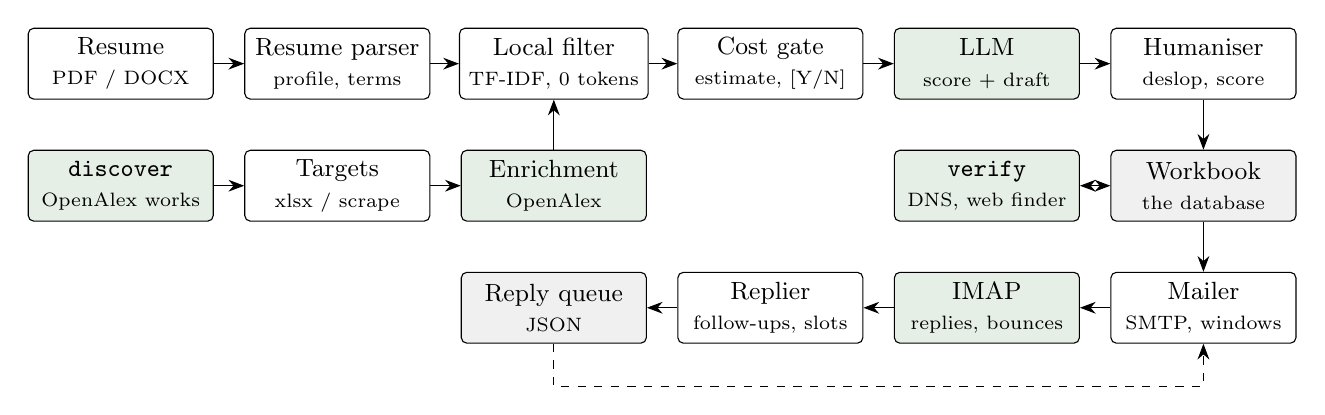
\begin{tikzpicture}[
  box/.style={draw,rounded corners=2pt,minimum width=2.35cm,minimum height=0.9cm,align=center,font=\small,fill=white},
  store/.style={box,fill=gray!12},
  ext/.style={box,fill=accent!12},
  >={Stealth[length=2mm]}, x=2.75cm, y=1.55cm]
  \node[box]   (resume)  at (0,0)  {Resume\\\scriptsize PDF / DOCX};
  \node[box]   (parse)   at (1,0)  {Resume parser\\\scriptsize profile, terms};
  \node[box]   (filter)  at (2,0)  {Local filter\\\scriptsize TF-IDF, 0 tokens};
  \node[box]   (gate)    at (3,0)  {Cost gate\\\scriptsize estimate, [Y/N]};
  \node[ext]   (llm)     at (4,0)  {LLM\\\scriptsize score + draft};
  \node[box]   (hum)     at (5,0)  {Humaniser\\\scriptsize deslop, score};
  \node[ext]   (disc)    at (0,-1) {\code{discover}\\\scriptsize OpenAlex works};
  \node[box]   (targets) at (1,-1) {Targets\\\scriptsize xlsx / scrape};
  \node[ext]   (enrich)  at (2,-1) {Enrichment\\\scriptsize OpenAlex};
  \node[ext]   (verify)  at (4,-1) {\code{verify}\\\scriptsize DNS, web finder};
  \node[store] (xlsx)    at (5,-1) {Workbook\\\scriptsize the database};
  \node[store] (queue)   at (2,-2) {Reply queue\\\scriptsize JSON};
  \node[box]   (replier) at (3,-2) {Replier\\\scriptsize follow-ups, slots};
  \node[ext]   (imap)    at (4,-2) {IMAP\\\scriptsize replies, bounces};
  \node[box]   (mail)    at (5,-2) {Mailer\\\scriptsize SMTP, windows};
  \draw[->] (resume) -- (parse);   \draw[->] (parse) -- (filter);
  \draw[->] (filter) -- (gate);    \draw[->] (gate) -- (llm);
  \draw[->] (llm) -- (hum);        \draw[->] (hum) -- (xlsx);
  \draw[->] (disc) -- (targets);   \draw[->] (targets) -- (enrich);
  \draw[->] (enrich) -- (filter);
  \draw[<->] (verify) -- (xlsx);   \draw[->] (xlsx) -- (mail);
  \draw[->] (mail) -- (imap);      \draw[->] (imap) -- (replier);
  \draw[->] (replier) -- (queue);
  \draw[->,dashed] (queue.south) -- ++(0,-0.35) -| (mail.south);
\end{tikzpicture}
\caption{Data flow. Shaded boxes hold persistent state; green boxes talk to external services.}
\label{fig:arch}
\end{figure}

Agnostos is a single Python package, \code{outreach}, driven by \code{outreach/cli.py}
(\code{python -m outreach.cli <command>}, or the \code{agnostos} console script). It needs Python
3.10 or newer. The core dependencies are \code{openpyxl}, \code{pdfplumber}, \code{python-docx},
\code{python-dotenv}, \code{openai}, \code{PyYAML}, \code{truststore}, \code{certifi} and
\code{httpx}. Playwright is optional (Mode~A scraping) and so is \code{ddgs} (metasearch for the
address finder).

\subsection{Components}

\begin{tabularx}{\linewidth}{@{}lX@{}}
\toprule
Module & Responsibility \\
\midrule
\code{config.py} & Settings from \code{.env} with defaults, provider table, model prices,
placeholder detection and \code{ConfigError}. \\
\code{resume\_parser.py} & PDF/DOCX/TXT to a \code{ResumeProfile}: sections, education,
interests, projects, achievements, domain-term keywords. \\
\code{excel\_io.py} & Mode~B ingestion with header detection and about 30 header aliases;
in-place result columns with backup; sending view; sidecar for locked workbooks. \\
\code{discover.py}, \code{batches.py} & Topic-driven discovery over the OpenAlex works index,
in resumable batches. \\
\code{scraper.py} & Mode~A: faculty-directory scraping with Playwright, falling back to plain
HTTP. \\
\code{enrich.py} & OpenAlex author resolution and recent-publication selection, with a cache. \\
\code{focus.py} & Keyword gate that keeps outreach on the student's field. \\
\code{matcher.py} & The local TF-IDF matcher and candidate filter. \\
\code{llm.py} & Cost estimate, \code{[Y/N]} gate, one call per professor, capability
negotiation, body repair, humaniser integration. \\
\code{humanize.py} & Deterministic deslop, AI-tell score, hard-claim and self-funding
detection, rewrite prompt. \\
\code{verify.py} & Address checks (syntax, DNS, name match) and the web address finder. \\
\code{recheck.py} & Is the person still publishing, and still at this institution? \\
\code{mailer.py}, \code{schedule.py} & SMTP dispatch, throttling, local send windows,
\code{--at} start times. \\
\code{replies.py}, \code{replier.py} & IMAP reply classification; whole-thread reading and
follow-up drafting. \\
\code{gcal.py} & Meeting-slot proposal and tentative calendar holds. \\
\code{legacy.py}, \code{replace.py} & Letters to eminent researchers; replacing bounced
contacts with a colleague. \\
\code{mailbox.py}, \code{convoview.py}, \code{stats.py}, \code{dashboard.py} & Sent-folder
archiving, the conversation page, funnel statistics and a console dashboard. \\
\code{tls.py} & One TLS context for HTTPS, SMTP and IMAP. \\
\bottomrule
\end{tabularx}

\subsection{The pipeline in six steps}
\code{run} prints six numbered steps: (1) parse the resume; (2) acquire targets from the
workbook (Mode~B) or by scraping (Mode~A), dropping rows already sent and, when \code{FOCUS} is
on, rows outside the student's field; (3) enrich from OpenAlex; (4) apply the local filter;
(5) estimate cost, ask for confirmation, then call the model once per selected professor;
(6) write results back. \code{discover} and \code{verify} run before \code{run} when the
student starts from a topic rather than a list; \code{send}, \code{check-replies} and
\code{replies} run after it.

%====================================================================
\section{Resume parsing}
%====================================================================

\code{parse\_resume} reads PDF (pdfplumber, \code{x\_tolerance=1}), DOCX or plain text.

\paragraph{Glued text repair.} Some PDF extractors drop spaces (\code{DeepLearning}). Let
$L$ be the number of letters, $S$ the number of spaces and $\bar w$ the mean word length. The
text is treated as glued when
\[
  \frac{S}{L} < 0.10 \quad\text{or}\quad \bar w > 11 ,
\]
and only then are spaces re-inserted at lower-to-upper case boundaries, around short joiner
words (\code{in}, \code{of}, \code{at}, \ldots), between letters and digits, and after
punctuation. The mean-word-length test is the decisive one, because normal English averages
about five to seven characters per token.

\paragraph{Sections.} A line is a section heading when its lower-cased letters fully match one of
the patterns for education, interests, projects, skills, achievements or experience, and it is
either upper-case or shorter than 45 characters. Other short upper-case lines of at most six
words open an unnamed section, so their content is not attached to the previous one.

\paragraph{Projects.} Lines that start with a top-level bullet glyph open a project; following
lines become its bullets; \code{Advised by \ldots} is captured as the advisor. Resumes without
bullet glyphs fall back to a title heuristic: a line of at most 80 characters and 12 words that
starts with a capital, has no terminal punctuation and has at least 60\% of its longer words
capitalised.

\paragraph{Keywords.} The parser carries a fixed vocabulary of about 120 domain terms
(\code{DOMAIN\_TERMS}: methods, physics subfields, tools). The keyword list is every domain term
present in the text, followed by other non-stop-word tokens longer than three characters that
occur at least twice, capped at 45. \code{skills} is the list of domain terms present (up to
30). \code{summary\_block()} turns the profile into a block of at most 2\,400 characters, with
up to four projects of at most 420 characters each, for the language model.

%====================================================================
\section{Target acquisition}
%====================================================================

\subsection{Mode B: an existing workbook}
Every sheet is scanned. The header row is the row among the first eight with the most cells that
match a known header alias (\code{Professor Name}, \code{Email}, \code{Affiliation},
\code{Research Interests}, \ldots). Sheets without a name column are skipped, so a
``Funding Programmes'' tab is ignored. Columns that match no alias are folded into the notes
field as \code{header: value}, which the model still sees. Rows are de-duplicated by email, or by
name and institution when there is no email.

\subsection{Mode A: directory scraping}
\code{scraper.py} drives Chromium through Playwright. It removes the common automation tells
(\code{navigator.webdriver}, plugins, WebGL vendor, \code{chrome.runtime}), randomises viewport,
locale, timezone and device scale per browser context, and moves the mouse along smoothstep
paths, $e(t) = t^2(3-2t)$, with random dwell times and scrolls. A page counts as blocked if one of
the hard challenge markers appears in its first 6\,000 characters, or if a softer marker appears
and the visible text is at most 2\,500 characters long. A blocked page is waited out once and then
retried with a fresh context (and a fresh proxy exit, if a proxy is configured).
\code{robots.txt} is honoured unless \code{RESPECT\_ROBOTS=false}; CAPTCHAs are not solved.
Delays between pages are uniform in $[4, 11]$\,s by default. Names are extracted around
academic titles and around email addresses (including \code{[at]}/\code{(dot)} obfuscation),
generic office mailboxes are dropped, and when a directory hides addresses the scraper follows
each person's profile link and matches the address by surname. Without Playwright it falls back
to plain HTTP.

\subsection{Topic focus}
With \code{FOCUS=true} (the default), \code{run} and \code{send} only process rows whose
research area, institution, department, recent works and topics match \code{FOCUS\_KEYWORDS}
(physics and high-energy physics stems by default). Let $h$ be the number of
\emph{distinct} keyword matches. A single hit next to an off-field marker (clinical, cancer,
protein, marketing, \ldots) does not count:
\[
  \text{in\_focus} = (h \ge 2) \;\lor\; (h = 1 \land \lnot\,\text{off\_field}) .
\]

%====================================================================
\section{Discovery from a research topic}\label{sec:discover}
%====================================================================

\code{discover} builds a list of professors without the student naming any university. It
searches the OpenAlex \emph{works} index for each topic and credits the people in the positions
that matter.

\subsection{Which papers count}
Each page requests 100 works with the filter
\code{from\_publication\_date:<since>-01-01}, \code{type:article}, \code{has\_doi:true}, the
selected countries, and institution types \code{education|facility}. Countries are resolved from
named groups (\code{europe}, \code{dach}, \code{nordics}, \code{usa}, \ldots) or ISO codes, with
\code{uk} mapped to \code{gb}.

\paragraph{Mega-collaborations.} A work with more than 15 authorships is discarded. A
2\,000-author detector paper names everyone and says nothing about who works on what.

\paragraph{Relevance floor.} The first page of each topic fixes an anchor: the highest
OpenAlex \code{relevance\_score} seen, $r_{\max}$. A work is kept only if
\[
  r \ge \rho \, r_{\max}, \qquad \rho = 0.1 .
\]
Results come best-first, so once an entire page is below the floor the topic is marked
exhausted.

\paragraph{Field anchoring.} Free-text search matches words, not meaning: ``geometric deep
learning'' also returns dentistry papers about tooth geometry. On the first page the 30 most
relevant works are grouped by their primary-topic \emph{field}, and a field is a home field when
it holds at least 15\% of them. Later works outside the home fields are ignored. Nothing about
subjects is hard-coded; each topic learns its own fields.

\subsection{Crediting authors}
For each kept work, only the \emph{first} and \emph{last} authors are credited, and only if they
have an institution with a ROR id in one of the selected countries. Each candidate accumulates:
$n$, the number of matching papers; $\ell$, how many of those had them as last author; $y$, the
newest publication year; their titles (up to six) and topics. After every page, newcomers are
hydrated in batches of 50 from the OpenAlex author records to obtain the h-index $h$ and the
works count $W$. A candidate is \emph{senior} when
\[
  h \ge 8 \quad\text{and}\quad W \ge 20
\]
(\code{--min-h-index}, \code{--min-works}). This gate removes first-year PhD students who
happened to be first author.

\subsection{Ranking}
Senior candidates are ranked by
\[
  s = n + 0.6\,\ell + 2\,\max\!\Bigl(0,\, 1 - \frac{Y - y}{5}\Bigr) + \frac{\min(h, 60)}{60},
\]
where $Y$ is the current year. Repeat appearances dominate (someone in four matching papers is
working on the topic), last-author position adds weight, recency decays linearly to zero over
five years, and the h-index contributes at most one point.

\paragraph{Top universities.} With \code{--top-universities N}, the region's universities are
ranked by the number of papers since \code{--since} with more than 50 citations, grouped by
institution and filtered to type \code{education} in the selected countries. This is a
field-agnostic proxy for reputation. Discovery then only queries papers from those institutions
(via \code{authorships.institutions.lineage}, so a lab inside a university counts), and the sort
key gains a prestige bonus. For a candidate at the university of rank $k$ among $R$,
\[
  s' = s + 5\,w \Bigl(1 - \frac{k-1}{R}\Bigr),
\]
with $w$ the prestige weight (\code{--prestige-weight}, default 1). The top-ranked university
adds $5w$, sliding towards zero for the last one. Universities named with
\code{--also-universities} are resolved by OpenAlex institution search and inserted at position
$\min(R, 10)$ of the ranking.

\subsection{Batches}\label{sec:batches}
The total count $C$ is split over $K$ batches by integer division,
\[
  C = qK + m, \qquad \text{quota}_i = q + [\,i \le m\,] ,
\]
and topics are assigned round-robin. A reused topic continues from the OpenAlex cursor the
previous batch reached, so it finds new people rather than the same ones. A batch pages until it
has its quota of senior researchers, the topic is exhausted, or it reaches the page cap (40 by
default). A shortfall is carried into the next batch's quota.

No one is added twice: every batch skips OpenAlex ids taken by earlier batches and by the output
workbook, and names are compared through an order- and accent-insensitive key (NFKD fold to
ASCII, lower-case, words of two or more letters, sorted), so \emph{Plehn, Tilman} equals
\emph{Tilman PLEHN}. Progress is stored in \code{<output>.batches.json} after each batch, keyed by
a fingerprint: the first 12 hex digits of the SHA-1 of the JSON-encoded topics, count, batches,
sorted countries, since-year, h-index and works thresholds, plus any non-default options that
change which papers qualify. The page cap and \code{--exclude} lists are deliberately not
hashed, so raising the cap continues a run instead of restarting it. Each row receives the
homepage from the ROR record of the person's institution, which later seeds the address search.

%====================================================================
\section{OpenAlex enrichment}
%====================================================================

For each professor, \code{enrich.py} searches OpenAlex authors by name (titles stripped, five
results). The first result whose affiliations or last known institutions contain a word of four
or more letters from the stated institution (ignoring \emph{university}, \emph{institute} and
\emph{college}) wins; otherwise, in non-strict mode, the top hit is used. Only confirmed matches
are cached, so a rate-limited miss is retried next time and a namesake is never cached.

The professor's works are then fetched newest first, $\max(6k, 25)$ of them for $k = 4$
publications per author (\code{OPENALEX\_WORKS}). Works with more than 15 authors are dropped.
The rest are sorted by the key
\[
  \bigl(-[\text{first or last author}],\; -\text{year}\bigr),
\]
de-duplicated on the first 80 characters of the normalised title, and the first $k$ are kept
as \code{title (year) - abstract}, where the abstract is rebuilt from OpenAlex's inverted index
and cut to 180 characters. Topic names (up to eight) become the professor's concepts. A 429
response sets a flag that stops further calls for the run; the pipeline continues with the text
it already has.

%====================================================================
\section{The local matcher}\label{sec:matcher}
%====================================================================

The matcher decides, without spending a token, which professors are worth a model call.

\subsection{Text normalisation and features}
Text is lower-cased and passed through a synonym layer of regular expressions (for example
\code{hep}, \code{lhc}, \code{atlas}, \code{cms}, \code{collider} $\to$ \emph{high-energy
physics}; \code{gnn}, \code{geometric deep learning} $\to$ \emph{graph neural network};
\code{pinn}, \code{physics-informed} $\to$ \emph{scientific machine learning}). Tokens are
runs of at least three characters that start with a letter and continue with letters, digits,
\code{+}, \code{\#} or \code{-}; stop words are removed. The feature multiset of a text is its
unigrams plus its adjacent bigrams. The professor side uses only text specific to that person
(research area, notes, fit note, recent works, OpenAlex concepts) and deliberately excludes the
department, which in Mode~A is a constant inherited from the source page.

\subsection{TF-IDF cosine}
Let the corpus be the $N_p$ professors plus the applicant profile, $N = N_p + 1$ documents. For a
term $t$ with document frequency $\mathrm{df}(t)$,
\[
  \mathrm{idf}(t) = \ln\frac{N + 1}{\mathrm{df}(t) + 1} + 1 ,
\]
and terms outside the corpus get $\mathrm{idf} = 2$. For a document with term counts $c_t$,
\[
  w_t = \frac{c_t}{\sum_u c_u}\,\mathrm{idf}(t)\,\beta_t, \qquad
  \beta_t = \begin{cases} 2.5 & t \in \text{DOMAIN\_TERMS} \\ 1 & \text{otherwise,}\end{cases}
\]
and the vector is $L_2$-normalised. The similarity is the cosine
$\cos = \sum_t \hat a_t \hat b_t$ between the profile vector $\hat a$ and the professor vector
$\hat b$. Computing IDF over the actual list matters: in a list of physicists the word
\emph{physics} is in every row and is correctly discounted.

\subsection{Saturating domain-term bonus}
Professor rows are often one-line topic strings, so coverage of the whole resume vocabulary would
be the wrong measure. Instead, let $M$ be the set of domain terms present in the profile that also
appear in the professor's normalised text, and
\[
  H = \sum_{t \in M} \begin{cases} 1.6 & t \text{ is a multi-word phrase} \\ 1.0 & \text{otherwise}\end{cases},
  \qquad
  \tau = 1 - e^{-0.5 H}.
\]
$\tau$ rewards absolute hits and saturates: one single-word hit gives $0.39$, two give $0.63$,
one phrase plus one word gives $0.73$.

\subsection{Combined score and selection}
\[
  \text{score} = 0.45\,\min(2.5\cos,\, 1) + 0.55\,\tau ,
\]
rounded to four decimals, and $0$ when the professor text is shorter than 12 characters.
Professors are sorted by score and then filtered in order:
\begin{enumerate}
  \item no email address $\to$ \code{skipped: no email};
  \item score below \code{MIN\_LOCAL\_SCORE} (default $0.25$) $\to$ skipped;
  \item no research signal, meaning no recent works and fewer than 30 characters of personal text
        $\to$ skipped, because a ``personalised'' email written from a directory stub is generic
        and wastes tokens;
  \item over the \code{MAX\_PROFESSORS} cap (default 50) $\to$ skipped;
  \item otherwise selected.
\end{enumerate}
\code{--skip filter} bypasses steps 2 and 3 but still requires an email and applies the cap.
The matched domain terms are passed to the model as ``local keyword overlap''.

%====================================================================
\section{Language-model evaluation and drafting}
%====================================================================

\subsection{One call per professor}
Each selected professor gets exactly one Chat Completions call that returns \emph{both} the
acceptance estimate and the email, as a JSON object with the fields \code{probability},
\code{justification}, \code{subject} and \code{body}. The system prompt contains the applicant
profile, availability and funding stance, a calibration rubric (80--100 near-perfect overlap with
a funded route, 60--79 strong, 40--59 adjacent or unclear funding, 20--39 weak, 1--19 wrong
field), honesty rules, a list of banned phrases and the email rules (130--180 words, salutation,
three or four short paragraphs, one specific thing from the professor's own recent work, one
thing the student built, one clear ask, plain text). Because it is identical for every
professor, providers with automatic prompt caching bill it at the cached rate after the first
call. The user message is the professor's context block, capped at 900 characters (name,
institution, department, research area, up to four recent works, up to eight topics, funding
and route fields, matched terms).

The returned probability is clamped to $[1, 100]$. The body is repaired before anything else:
a salutation \emph{Dear Prof./Dr. Surname} is added if missing (the title is \emph{Prof.} only if
the row's name starts with Prof/Professor), a short trailing sign-off is separated, and a
single block of four or more sentences is split into chunks of
$\max(2, \lceil n/3 \rceil)$ sentences.

\subsection{Token and cost estimate}
Before any paid call, the tool prints an estimate and asks \code{[Y/N]}. Tokens are approximated
as
\[
  T(x) = \max\bigl(1,\, \lfloor |x|/4 \rfloor + \#\text{newlines}(x)\bigr) .
\]
With $n$ professors, system prompt $S = T(\text{system})$ and user messages $u_i$: if the
provider caches prompts and $S \ge 1024$ (the minimum cacheable prefix),
\[
  \text{cached} = S\,(n - 1), \qquad \text{fresh} = S + \textstyle\sum_i u_i ;
\]
otherwise $\text{cached} = 0$ and $\text{fresh} = nS + \sum_i u_i$. Output is estimated as
$n \lfloor 0.55\,B \rfloor$, where $B$ is the output budget (\code{MAX\_OUTPUT\_TOKENS}, default
1\,100, raised to at least 4\,000 for reasoning models whose names start with \code{o} or
\code{gpt-5}). If the rewrite pass is enabled, $r = \max(1, \lfloor n/3 \rfloor)$ rewrites are
assumed, adding $r\,(T(\text{rewrite prompt}) + 260)$ input and $230\,r$ output tokens. With
prices $(p_{\text{in}}, p_{\text{cached}}, p_{\text{out}})$ in USD per million tokens,
\[
  \text{cost} = 10^{-6}\bigl(p_{\text{in}}\,\text{fresh} + p_{\text{cached}}\,\text{cached}
  + p_{\text{out}}\,\text{out}\bigr).
\]
Free-tier providers (Groq) are priced at zero. Unknown models fall back to the \code{gpt-4.1}
price $(2.00, 0.50, 8.00)$. During the run the actual cost is computed the same way from the
reported usage (cached tokens subtracted from prompt tokens), and the run stops issuing calls
once it reaches \code{BUDGET\_USD} (default \$5).

\subsection{Capability negotiation}
Gateways differ in what they accept. The request starts optimistic: strict JSON-schema
structured output, \code{max\_completion\_tokens} and an explicit temperature (0.4 for drafting;
omitted for reasoning models). On a \code{BadRequestError} the client switches off the next
capability in the fixed order
\[
  \texttt{json\_schema} \to \texttt{json\_object} \to \texttt{max\_completion\_tokens}
  \;(\text{use } \texttt{max\_tokens}) \to \texttt{temperature},
\]
and retries. Downgrades are remembered for the rest of the run and do not use up retries. A
response cut off with \code{finish\_reason = length} doubles the output budget, up to 16\,000,
and retries. Other transient errors are retried up to three times with back-off $2^{a}$ seconds
after attempt $a$. Authentication, permission and not-found errors stop at once. Three
consecutive failed professors abort the run, so a broken key does not burn the whole list.
If structured output is unavailable, the parser strips code fences and falls back to the first
brace-delimited span.

%====================================================================
\section{The humanising layer}\label{sec:humanize}
%====================================================================

\subsection{Stage 1: deterministic deslop}
\code{deslop} applies three ordered substitution tables, case-insensitively: whole phrases
(``I hope this email finds you well'' is removed, ``I am writing to'' becomes ``I wanted to'',
``aligns with'' becomes ``lines up with''), overclaiming verbs swapped verb-for-verb
(\emph{achieved} $\to$ \emph{got}, \emph{demonstrated} $\to$ \emph{showed}, \emph{outperformed}
$\to$ \emph{was compared against}), and single words with the same part of speech
(\emph{utilise} $\to$ \emph{use}, \emph{furthermore} $\to$ \emph{also}, \emph{novel} removed). It
then drops the middle item of the first ``X, Y, and Z'' triad, turns em dashes into commas,
removes markdown and bullets, and fixes spacing and capitalisation. It is conservative on
purpose: it only makes substitutions that cannot break grammar, because a mangled sentence is
worse than a formal one.

\subsection{Stage 2: the AI-tell score}
For a draft $x$, each tell pattern $i$ with weight $w_i$ and $k_i(x)$ matches contributes
$w_i k_i(x)$:

\begin{center}
\begin{tabular}{@{}lr@{}}
\toprule
Tell & Weight \\
\midrule
Unverifiable result claim (hard claim, below) & 6 \\
Boilerplate greeting (``I hope this email finds you well'') & 5 \\
LLM vocabulary (delve, leverage, robust, seamless, \ldots) & 4 \\
Form-letter opener (``I am writing to'', ``I am reaching out'') & 4 \\
Overclaiming (achieved, demonstrated, novel, superior, \ldots) & 4 \\
Em dash; markdown or bullets; performed enthusiasm & 3 \\
Alignment clich\'e; three-item list & 3 \\
Formal connective (moreover, furthermore, thus, hence, therefore) & 2 \\
\bottomrule
\end{tabular}
\end{center}

\noindent If the draft has at least four sentences with word counts $\ell_j$, mean $\mu$ and
population variance $\sigma^2$, two rhythm terms are added: $+8$ if $\sigma^2 < 12$ (uniform
sentence length is a strong tell of machine text) and $+5$ if $\mu > 26$. The score is
\[
  A(x) = \min\Bigl(100,\; \sum_i w_i k_i(x) + 8\,[\sigma^2 < 12] + 5\,[\mu > 26]\Bigr).
\]

\paragraph{Hard claims} are matched separately: a percentage, ``improved/enhanced/boosted
(the) accuracy/performance/results'', ``beat(s) the baseline/state'', ``best-in-class'', or
``resulted in improved/enhanced/superior/better''. These cannot be softened safely.

\subsection{Stage 3: conditional rewrite}
A draft goes back to the model only when
\[
  A(\text{deslop}(x)) \ge \theta \quad\text{or}\quad \text{it contains a hard claim},
\]
with $\theta =$ \code{HUMANIZE\_THRESHOLD} $= 10$ and \code{HUMANIZE\_REWRITE=true}. The rewrite
uses temperature 0.8 (higher temperature reads less uniform) and a prompt that keeps every fact
and the salutation and sign-off, shortens to 120--180 words, varies sentence length and removes
claims of results. The rewritten body is repaired and deslopped again and is kept \emph{only if}
its score is no higher than the original's. A failed rewrite is never fatal. Any remaining hard
claim puts \code{UNVERIFIED CLAIM - review before sending} at the front of the \code{Review
Flags} column, and the final score is written to \code{AI-Tell Score}.

\subsection{Self-funding guard}
Unless \code{CAN\_SELF\_FUND} is set to yes, a sentence that offers to pay one's own travel, visa,
accommodation or living costs (a modal verb, a paying verb and a cost noun within a short
window, or ``self-fund'') and contains no negation is removed. Where such a sentence begins
with an availability clause (``I'm available for 8--12 weeks and can cover travel''), the
availability part is kept. The same check runs again in the mailer immediately before sending,
and a message that still contains an offer is skipped rather than sent.

%====================================================================
\section{Email verification and repair}\label{sec:verify}
%====================================================================

\subsection{Local confidence model}
\code{check\_email} starts from 100 points. An address that fails the shape check is
\emph{invalid}. If DNS shows the domain has neither MX nor A records, it is \emph{invalid}; if
the lookup itself fails, $10$ points are subtracted (a failed lookup is never treated as a bad
address). The local part is then compared with the person's name by $m = \text{name\_match} \in
[0,1]$:

\begin{center}
\begin{tabular}{@{}lll@{}}
\toprule
$m$ & Meaning & Penalty \\
\midrule
1.0 & a usual pattern (\code{first.last}, \code{flast}, \code{last}, \ldots) & 0 \\
0.9 & truncated surname, or initials plus a numeric id & $-10$ \\
0.75 & surname appears intact in another form & $-10$ \\
0.6 & only the given name appears & $-25$ \\
0.5 & short initialism & $-25$ \\
0.3 & letters plus digits that do not match the initials & $-35$ \\
0 & no relationship, or a generic mailbox (\code{info@}, \code{office@}) & $-55$ \\
\bottomrule
\end{tabular}
\end{center}

\noindent The variant set behind $m=1$ tries every trailing token as the surname, compound
surnames joined in several ways, and particles (\emph{van}, \emph{von}, \emph{de}) removed; all
names are accent-folded. If the person's own page was found on a different site, $20$ points are
subtracted; otherwise a free-mail domain costs $30$. An optional SMTP \code{RCPT} probe adds $10$
on acceptance and marks the address invalid on a definite 550/551/553, but it is off by default
because catch-all servers accept everything. The confidence is the result clamped to
$[0, 100]$, and the status is \emph{ok} when it is at least 70, \emph{suspect} otherwise.

\subsection{The web address finder}
With \code{--repair}, the finder reads pages about the person: their profile URL (only if it has
a real path, not a homepage), then the results of up to four search phrasings, beginning with
\code{"<name> email site:<host>"} when the institution host is known. Search goes through the
\code{ddgs} metasearch package, trying backends in turn (the last one that worked first),
with a hard deadline of $3t + 10$ seconds per call ($t = 15$\,s) because the library can hang;
DuckDuckGo's HTML endpoint is the last resort. Requests to any single host are spaced at least
1.5\,s apart across all worker threads. From each page the finder extracts plain, \code{mailto:},
\code{[at]}/\code{(dot)}-obfuscated, TYPO3 Caesar-shifted and Cloudflare XOR-encoded addresses,
and reads the first two pages of PDFs (papers print their authors' addresses).

Each address $e$ found on host $h$ is scored. It is discarded if $m(e) < 0.75$, if its local part
names a different given name than the person's, or if $m < 1$ and the address is on another
country's top-level domain. Otherwise
\[
  s(e) = m + b(e) + 0.5\,[\text{academic}] + 0.25\,[\text{profile page}],
\]
where the domain bonus $b(e)$ is
\[
  b(e) = \begin{cases}
    1.0 & \text{if the address domain is the same site as } h,\\
    0.75 & \text{else if it is the same site as the institution's ROR homepage},\\
    0.5 & \text{else if } m = 1 \text{ and the domain spells the institution},\\
    0 & \text{otherwise.}
  \end{cases}
\]
``Same site'' means equal or one a sub-domain of the other, and ``academic'' means not a known
free-mail host. If $m = 1$, the domain is academic and the same address was seen on two different
hosts, $s \leftarrow \max(s, 2)$: two unrelated sources agree. The best address wins, and the
search stops early once $s \ge 2$.

\subsection{Adoption rules}
A found address is only used when $s \ge 1.75$.
\begin{itemize}
  \item Row has no address (rows from \code{discover}): the found one becomes the suggestion with
        status \emph{suspect} and confidence $\min(90, \lfloor 55 + 15 s \rfloor)$.
  \item Row has a different address on another site: confidence is capped at 45 and the status
        becomes \emph{suspect}.
  \item Row has the same address: status \emph{ok}, confidence at least 95.
\end{itemize}
With \code{--apply}, the suggestion replaces the row's address only if the row had none or its
current address is not \emph{ok}; the row is then re-checked. A passing address is never
replaced, and the alternative stays in \code{Suggested Email} for a human to judge. Results with
$s \ge 1.75$ are cached; misses are not, because a miss is usually a blocked search engine. Rows
already sent are skipped unless \code{--include-sent} is given, and the mailer refuses rows marked
\emph{invalid} unless \code{--allow-unverified} is passed.

%====================================================================
\section{Professor recheck}
%====================================================================

\code{recheck} asks the question before address verification: is this person still publishing,
and still there? It reads the OpenAlex author record (by id when the row has one, otherwise by
a strict name search that only accepts a record whose affiliations match the row). With $Y$ the
current year and $y^\ast$ the latest year with at least one work:
\begin{itemize}
  \item \emph{inactive} if $Y - y^\ast \ge 3$;
  \item \emph{moved} if none of the last known institutions, nor any affiliation active in the
        last two years, matches the row's institution under any OpenAlex name, acronym or
        alternative name;
  \item \emph{active} otherwise; \emph{not found} when no record matches.
\end{itemize}
Institution names match loosely: after accent folding and removing generic words (university,
institute, of, \ldots), two names match if they share a word, if one word contains the other (for
words of four or more letters), or if a short word in one is an acronym of the other
(\emph{KIT} for Karlsruhe Institute of Technology). A row listing two places (``Nikhef / UvA'')
matches if either does. A failed lookup leaves the previous status untouched, and blank
Institution and OpenAlex ID cells are filled in from the record.

%====================================================================
\section{Sending}
%====================================================================

\subsection{Selection}
The mailer considers rows with a draft and an address whose \code{Send Status} is not
\emph{sent} (or \emph{review-sent} in review mode), and whose probability is at least
\code{--min-probability}. With \code{--top N} the rows are sorted by probability and the best $N$
are kept; \code{--limit} (default \code{DAILY\_SEND\_CAP} $= 25$) then caps real sends in this
run. With \code{FOCUS} on, off-field rows are excluded as in \code{run}.

\subsection{Recipient-local send windows}
A window \code{H1-H2} (minutes $[a, b)$, with $b > a$) is evaluated in the recipient's time
zone, derived from the Country column (ISO code or name). Countries spanning several zones use
an override (the US maps to New York, Australia to Sydney, Germany to Berlin, and so on);
others use the first \code{zone.tab} entry. A row may be sent at local time $t$ when
\[
  a \le 60\,t_h + t_m < b \quad\text{and}\quad (\text{weekday} \lor \texttt{--weekends}) .
\]
Otherwise the scheduler scans the next eight days for the first opening after $t$ and reports the
wait. Rows with no usable country are never held back. With \code{--wait}, the mailer closes the
SMTP connection and sleeps until the earliest opening across the queue; without it, held rows are
left for a later run. \code{--at} delays the start to a given local time (\code{HH:MM}, rolling to
tomorrow if already past, or a full date).

\subsection{Throttling and failure handling}
After each successful send the mailer waits a uniformly random time in
$[\code{SEND\_DELAY\_MIN}, \code{SEND\_DELAY\_MAX}] = [90, 240]$\,s, using the wall clock so a
sleeping laptop does not stretch the wait. If the wait exceeds 30\,s, the connection is closed
and reopened for the next message, because university relays drop idle sessions. Connecting is
tried three times with $15a$\,s pauses. A message that fails on a dropped connection is retried
once on a fresh one. After a failed message the mailer pauses $\min(30, 5k)$\,s for the $k$-th
consecutive failure, and three consecutive failures stop the run so the remaining rows stay
sendable.

\subsection{Never mailing twice}
\code{send --live} refuses to start if the workbook is open in Excel. Each result (status,
time, Message-ID) is written back to the workbook; if the file becomes locked during a run, the
updates are parked in \code{<workbook>.xlsx.pending-status.json} and merged on the next
successful write, with later updates for the same cell winning. Rows in the sidecar count as sent
for \code{send}, \code{verify} and \code{recheck}. Every attempt is also appended to
\code{output/send\_log.csv}. Dry runs never block a later real send.

\subsection{Messages}
Each message carries a fresh Message-ID on the sender's domain, an automatically appended
signature built from the resume, and the files listed in \code{ATTACHMENTS}. A copy is appended
to the IMAP Sent folder (\code{SAVE\_TO\_SENT}) so mail clients show complete threads.
\code{--review} mails each draft to the student instead, with the real recipient in the subject;
\code{--export} writes \code{.eml} files.

%====================================================================
\section{Replies and follow-ups}
%====================================================================

\subsection{Reply tracking}
\code{check-replies} logs into IMAP over TLS, selects each folder read-only and fetches with
\code{BODY.PEEK}, so nothing is marked as read. For each sent row it searches, since one day
before the earliest send, for mail from the professor's address and for mail whose
\code{In-Reply-To} or \code{References} header contains the stored Message-ID. Mail from
\code{mailer-daemon}/\code{postmaster} is matched to a row by the failed address quoted in the
notice. Each message is classified:
\begin{itemize}
  \item \emph{bounced}: sender or subject looks like a delivery-status notification;
  \item \emph{auto-reply}: an \code{Auto-Submitted} header other than \code{no},
        \code{X-Autoreply}/\code{X-Autorespond}, \code{Precedence} of auto\_reply/bulk/junk, or an
        out-of-office subject in one of several languages;
  \item \emph{replied}: anything else.
\end{itemize}
A row keeps the strongest result under the order $\text{bounced} < \text{auto-reply} <
\text{replied}$, so a later bounce never hides a real answer. A one-line snippet, stopping at the
first quoted line, goes into \code{Follow-up Notes}; notes typed by hand are kept.

\subsection{Drafting replies}
\code{replies} reads each whole thread (inbox, spam and Sent folders, plus the original email
from the workbook if Sent has no copy), orders it by date and asks the model to choose an action:
\emph{reply}, \emph{thank} (a 40--70 word gracious close) or \emph{none}. The prompt requires
every direct question to be answered, forbids invented facts (unknowns become
\code{[FILL: \ldots]}), and, when a professor says funding is unavailable, requires a reply that
keeps the door open instead of a thank-you. Drafts go to \code{output/reply\_queue.json} and are
only sent once approved. If a reply says something is attached, the CV is attached; if the file
is missing, the send fails rather than going out without the promised attachment.

\subsection{Funding follow-ups}
When a professor has raised funding and then gone quiet after the student's answer, each
\code{replies} run may draft another follow-up, at most \code{FUNDING\_FOLLOWUPS} $= 2$ per
thread, and only after \code{FOLLOWUP\_GAP\_DAYS} $= 2$ days of silence since the student's last
message. As soon as the professor writes again, the thread becomes a normal reply.

\subsection{Meeting slots}
The student's second message in a thread, and every funding follow-up, asks for a short call
(\code{MEET\_MINUTES} $= 20$) and offers three slots. \code{propose\_slots} walks forward day by
day from $t_0 = \text{now} + \code{MEET\_LEAD\_DAYS}$ (2 days) to $t_0 + 14$ days. For each
weekday not yet used it tries start times on a 30-minute grid inside the professor's hours
\code{MEET\_THEIR\_HOURS} (9--17 local) and takes the first start $s$ with end $e = s + d$ such
that
\begin{itemize}
  \item $s \ge t_0$ and $e$ is within the professor's hours;
  \item $[s, e]$ lies inside the student's hours \code{MEET\_MY\_HOURS} (13--23 in
        \code{MEET\_MY\_TZ}, Asia/Kolkata by default) on a single calendar day;
  \item $[s, e]$ overlaps no busy interval, where busy intervals are the slots already offered
        to other professors in the queue plus, if Google Calendar is connected, the calendar's
        free/busy blocks.
\end{itemize}
At most one slot is taken per day, so the three slots fall on different weekdays. When the
email is sent, each slot becomes a tentative \emph{HOLD} event on the student's calendar.

\subsection{Resending from a second account}
\code{resend} re-delivers the \emph{exact} original subject and body through a second SMTP
account to rows that were sent but bounced or got no answer, skipping replied and auto-replied
rows, addresses known to be invalid, rows already resent (from the send log and a
\code{Resent At} column) and rows first mailed fewer than \code{RESEND\_MIN\_DAYS} $= 4$ days
earlier. Bounced rows go first, and \code{RESEND\_DAILY\_CAP} $= 100$ limits sends per day. The
original send columns are never changed.

%====================================================================
\section{Letters to leading researchers}
%====================================================================

\code{legacy} writes a different kind of email: a short letter from an aspiring scientist to a
high-impact researcher. Let $A$ be the current year minus two. For each topic it takes the 100
most-cited works with more than 200 citations published since $A - 10$, collects the first 12
authors of each, hydrates up to 200 of them, and walks them in descending h-index order, keeping
authors with $h \ge 60$ (\code{--min-h}) and at least two works since $A$ (still active), up to
eight per topic. People named with \code{--include} are added from an author search. A
candidate is kept only if its topics and recent titles contain at least two distinct physics
terms and no off-field marker. Recent work is taken from papers with at most 12 authors, so a
letter never credits someone with a 3\,000-author paper. Addresses come from the same finder as
\code{verify}, and are rejected when the domain is in another country, is a \code{.edu} for a
non-US institution, or shares no word, initials or abbreviated label with the institution. The
model may only name a summer route from a fixed list (CERN, DESY, DAAD WISE, Mitacs, Charpak,
\ldots) chosen from the institution and country. Each letter must be approved in the workbook
before it is sent; \code{--approve-all} only covers addresses the finder verified.

%====================================================================
\section{Security and privacy}
%====================================================================

\begin{itemize}
  \item \textbf{Secrets.} All credentials live in \code{.env}; \code{.env},
        \code{credentials.json} and \code{client\_secret*.json} are git-ignored. Values still
        equal to the \code{.env.example} placeholders are treated as unset and reported as a
        single \code{CONFIG:} message before any network call.
  \item \textbf{Personal data.} Workbooks, caches, logs, the reply queue and the Google token
        are written to \code{output/}, which is git-ignored, as are per-run failure reports.
  \item \textbf{TLS.} HTTPS, SMTP and IMAP share one context that never disables verification. It
        prefers \code{SSL\_CERT\_FILE}/\code{REQUESTS\_CA\_BUNDLE}, then the operating-system
        store through \code{truststore}, then \code{certifi}. The one exception is the optional
        Playwright scraper, whose browser context ignores HTTPS errors on directory pages.
  \item \textbf{Mailbox access.} IMAP is used read-only for reply tracking. The Google Calendar
        scope is the calendar scope only, and the OAuth token is cached in \code{output/}.
  \item \textbf{Politeness.} Scraping honours \code{robots.txt} by default, never solves
        CAPTCHAs and waits 4--11\,s between pages. The address finder spaces requests per host,
        and OpenAlex calls are spaced 0.12--0.15\,s apart; enrichment stops on a 429.
  \item \textbf{What gets sent.} Nothing is sent without \code{--live}. The cost gate, hard-claim
        flags, the self-funding guard, the invalid-address block and the consecutive-failure
        abort all sit between a draft and a professor's inbox.
\end{itemize}

%====================================================================
\section{Interfaces}
%====================================================================

\begin{description}
  \item[CLI.] \code{profile}, \code{models}, \code{run}, \code{discover}, \code{verify},
        \code{recheck}, \code{send}, \code{stats}, \code{check-replies}, \code{replies},
        \code{conversations}, \code{archive-sent}, \code{resend}, \code{legacy},
        \code{replace-failed}, \code{calendar-auth} and \code{tls-check}.
  \item[Workbook.] Result columns appended in place (after a timestamped backup):
        \code{Local Match Score}, \code{Probability of Acceptance}, \code{Probability
        Justification}, \code{Email Subject}, \code{Custom Email Draft}, \code{AI-Tell Score},
        \code{Review Flags}, \code{Email Status}, \code{Email Confidence}, \code{Email Notes},
        \code{Suggested Email}, \code{Profile Status}, \code{LLM Status}, \code{Send Status},
        \code{Sent At}, \code{Reply Status} and \code{Follow-up Notes}. Re-running refreshes
        these columns instead of duplicating them, and blank model results never overwrite cells
        edited by hand.
  \item[Files.] \code{output/send\_log.csv}, \code{output/reply\_queue.json},
        \code{output/conversations.html}, \code{<output>.batches.json} and the OpenAlex,
        discovery and address caches.
  \item[Providers.] Any OpenAI-compatible endpoint: Groq (default, \code{openai/gpt-oss-120b}),
        OpenAI (\code{gpt-4.1}) or a gateway set by \code{OPENAI\_BASE\_URL}.
\end{description}

%====================================================================
\section{Testing}
%====================================================================

Two suites run on a fresh clone with no \code{.env} and no API key, using synthetic fixtures.
\code{tests/smoke\_test.py} is fully mocked: resume parsing, Excel round-trips, filter
behaviour, cost arithmetic on free and paid providers, a mocked model pass, abort on repeated
failures, body repair, the humaniser, idempotent column writes, attachments, resume safety for
interrupted sends, \code{.eml} export, scraper extraction and block detection, address
verification, batch planning and fingerprints, institution matching for \code{recheck}, and the
rule that \code{--apply} never replaces a passing address. \code{tests/openai\_stub\_test.py} runs
the real \code{openai} SDK against a local HTTP stub and checks request shape, cached-token
accounting, temperature omission for reasoning models, truncation handling and capability
downgrade. CI runs both on Python 3.10, 3.12 and 3.13.

%====================================================================
\section{Limitations}
%====================================================================

\begin{itemize}
  \item The acceptance probability is the language model's guess against a rubric, not a
        statistical estimate. It is useful for ordering, not as a frequency.
  \item The local matcher is lexical. Synonyms and the domain vocabulary help, but two
        descriptions of the same work in different words can still score low. The vocabulary
        and the default focus keywords lean towards physics and machine learning.
  \item OpenAlex author disambiguation is imperfect: one person can be split across several ids
        and a namesake can be merged in. Discovery keeps one record per name; recheck uses
        strict institution matching to limit the damage.
  \item The address finder depends on public search engines that block scrapers unpredictably.
        A miss is usually a blocked search, not proof that no address exists. Repair takes 20--40
        seconds per professor.
  \item Reply classification is rule-based and can mislabel unusual auto-replies.
  \item Time zones come from the country, so a professor in a country with several zones is
        scheduled in its main one.
  \item The token estimate uses four characters per token and a fixed rewrite rate; the budget
        cap itself uses the provider's reported usage.
\end{itemize}

%====================================================================
\section{Outlook}
%====================================================================

Natural next steps are an embedding-based matcher that runs locally beside the lexical one, a
field-neutral default vocabulary derived from the resume itself, per-institution time zones from
ROR coordinates, and learning the reply classifier from the student's own labelled threads. A
hosted web version of the tool is developed separately as Agnostos~v3.

\vspace{1em}
\noindent\textit{Agnostos is MIT-licensed. It drafts; the student reads, edits and signs every
email.}

\end{document}
